\section{Atacs de suplantació d'identitat}
\subsection{Atacs de ARP Spoofing}
\label{sec:spoofing}
En aquest apartat s'expliquen atacs de suplantació d'identitat que poden ser realitzats contra una xarxa MQTT. Aquests atacs tenen com a objectiu suplantar la identitat d'un client legítim per tal d'enviar missatges al broker MQTT o rebre'n, fent que el broker no pugui distingir entre clients legítims i clients maliciosos. També el fet de modificar informació legítima a través de sistemes de Man In The Middle. 

Primer de tot, s'ha estudiat el funcionament d'atacs de ARP Spoofing, per entendre'ls és necessari conèixer el protocol ARP en profunditat.

El Protocol de Resolució d'Adreces (ARP) és un mecanisme fonamental en xarxes IP que permet als dispositius d'una xarxa local associar adreces IP amb adreces MAC corresponents. Quan un dispositiu necessita enviar un paquet a una adreça IP dins de la seva mateixa xarxa local, emet una petició ARP a través de difusió (broadcast), sol·licitant quina adreça MAC està associada a aquella IP. El dispositiu propietari d’aquesta adreça IP respon amb la seva adreça MAC, i aquesta informació queda temporalment registrada a la taula ARP del dispositiu que ha fet la sol·licitud. Tot i la seva simplicitat i eficiència, ARP no incorpora cap mecanisme d'autenticació, la qual cosa el fa vulnerable a diversos tipus d’atacs, entre els quals destaca l’ARP spoofing.

L’ARP spoofing, també conegut com a ARP poisoning, és una tècnica d’atac que aprofita la manca de verificació en el protocol ARP per introduir entrades falses en les taules ARP dels dispositius de la xarxa. L’objectiu principal és enganyar aquests dispositius perquè associïn una adreça IP legítima (habitualment la del gateway o la d’una víctima específica) amb l’adreça MAC de l’atacant. Això permet a l’atacant interceptar el tràfic que, en condicions normals, es dirigiria directament al gateway o a un altre dispositiu. D’aquesta manera, es crea una situació de tipus Man-in-the-Middle (MitM), en què l’atacant pot monitoritzar, modificar o redirigir el tràfic entre dispositius.


El funcionament bàsic d’un atac ARP spoofing es pot resumir en els passos següents:

\begin{itemize}
    \item L’atacant envia respostes ARP falsificades a la víctima, fent-se passar pel gateway de la xarxa.
    \item Simultàniament, envia respostes ARP falsificades al gateway, fent-se passar per la víctima.
    \item Tant la víctima com el gateway actualitzen les seves taules ARP amb les associacions falses proporcionades per l’atacant.
    \item A partir d’aquest moment, el tràfic entre ambdós dispositius es redirigeix a través de l’atacant, que pot actuar com a passarel·la transparent (forwarder) o bé manipular els paquets segons el seu objectiu.
\end{itemize}

En aquest treball, inicialment s'ha utilitzat l'eina arpspoof del paquet dsniff ( \ref{sec:ARPSpoof} ) per realitzar l'atac ARP spoofing. Aquesta eina permet enviar respostes ARP falsificades a la víctima i el broker o el gateway, fent que ambdós dispositius actualitzin les seves taules ARP amb les associacions falses proporcionades per l'atacant tal com s'ha explicat anteriorment.

Un exemple d'execució utilitzada on client real víctima té l'adreça IP 192.168.0.41 i és:

\begin{lstlisting}[language=bash, caption={Execució Arpspoof}, label=lst:arpspoof]
    arpspoof -i wlp42s0 192.168.0.41
\end{lstlisting}

Amb aquesta execució aconseguim que els missatges que envia el broker MQTT al client real es redirigeixin a l'atacant. D'aquesta manera, si el client està subscrit a un tòpic concret, podem fer que l'atacant rebi aquests missatges, com per exemple podrien ser mesures de ritme cardíac o pressió sanguínia que deixen d'arribar a un monitoritzador mèdic. 

Però, aquest atac és fàcilment detectable. Per això, cal implementar un atac bidireccional, fent que tant el broker com el client enviïn els missatges a l'adreça MAC de l'atacant, generant una situació de MITM. Ho podem aconseguir amb una execució similar a la següent on s'afegeix l'adreça IP del broker MQTT 192.168.0.40 amb el paràmetre -r:

\begin{lstlisting}[language=bash, caption={Execució Arpspoof bidireccional}, label=lst:arpspoof_bidireccional]
    arpspoof -i wlp42s0 -t 192.168.0.41 -r 192.168.0.40
\end{lstlisting}

Per al perfeccionament de l'atac APR Spoofing, he utilitzat l'eina Bettercap que permet personalitzar les estratègies d'ARP spoofing i fer que l'atac sigui més difícil de detectar per un IDS i així poder generar trànsit més realista. 

Una de les configuracions addicionals que podem utilitzar amb aquesta eina és l'opció \textit{mac.changer} per fer que l'atacant canviï la seva adreça MAC de forma aleatòria, fent més difícil la detecció de l'atac per mac repetida. També amb l'opció "arp.spoof.targets" els paquets ARP van dirigits aquests dispositius en concret en comptes de a tota la xarxa, de manera que no es genera tant trànsit broadcast que és molt més detectable. Un exemple d'execució és:

\begin{lstlisting}[language=bash, caption={Execució Bettercap}, label=lst:bettercap]
bettercap -iface wlp42s0 -eval \"mac.changer on; set arp.spoof.internal true; set arp.spoof.targets 192.168.0.41,192.168.0.40; arp.spoof on\"
\end{lstlisting}

\subsection{Atacs de MITM}
\label{sec:MITM}
Un cop es disposa de l'atac d'ARP spoofing implementat, es pot utilitzar per a realitzar diversos atacs de Man In The Middle (MITM). 

El primer atac de MITM implementat, es basa a desplegar un broker MQTT mitjançant Mosquitto. Al desplegar un broker entremig, el que aconseguim és que el client cregui que està enviant els missatges al broker legítim, però en realitat els missatges són enviats a l'atacant i aquest pot respondre a aquest pot rebre i publicar en el mateix tòpic al qual el client està publicant o subscrivint-se.

Això permet a l'atacant interceptar i manipular els missatges que es transmeten entre el client i el broker, però trenca la connexió, és a dir, el broker legítim no rep ni envia missatges al client, per tant, és fàcilment detectable.

Per a l'obtenció d'aquest atac, és necessari implementar un ARP spoofing de l'adreça MAC del broker, l'adreça del client no és necessària si l'objectiu és comprometre el client IoMT. 

  \begin{figure}[H]
    \centering
    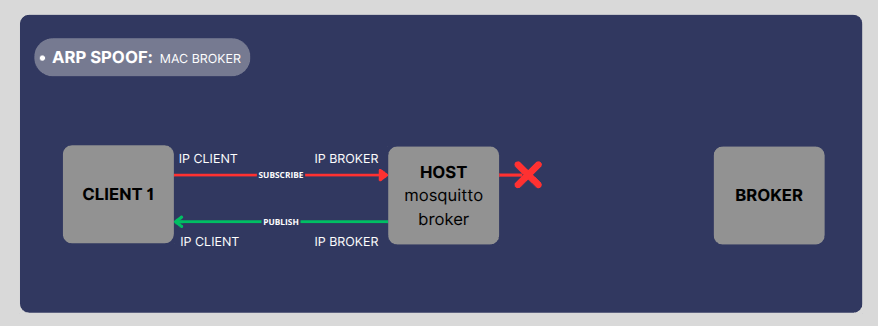
\includegraphics[width=1\textwidth]{img/mitmbroker.png}
    \caption{Esquema del trànsit generat per l'atac de Man In The Middle mitjançant un broker MQTT desplegat per l'atacant. S'observa un tall de la connexió entre el client i el broker legítim.}
    \label{fig:MITMbroker}
  \end{figure}

Una altra tècnica de MITM implementada, és l'ús d'un proxy TCP. Aquest actua com a intermediari entre el client i el broker. D'aquesta manera, intercepta el trànsit MQTT que rep i el reenvia al broker legítim, i viceversa. En aquest cas el resultat és que el broker legítim rep les peticions del client amb l'adreça IP del proxy com a origen i, per tant, el broker i el client poden intercanviar el \textit{handshake TCP} i el \textit{handshake MQTT Connect} correctament, però amb l'adreça IP del proxy com a origen i destí dels missatges.

Aquest mètode és més eficient que el desplegament d'un broker MQTT, ja que no trenca la connexió entre el client i el broker legítim, però sí que permet a l'atacant interceptar i manipular els missatges que es transmeten entre ambdues parts i alhora dificultar la seva detecció. 

Per a la implementació d'aquest atac, és necessari haver perpetrat un atac d'ARP spoofing de l'adreça MAC del broker, ja que en substituir la IP del client per la del proxy atacant, la connexió es farà a aquesta IP i el broker legítim li enviarà els paquets sense necessitat de suplantar l'adreça IP del client.

Per al desplegament del proxy, s'ha utilitzat l'eina \textit{Mitmproxy} ( \ref{sec:MITMProxy} ). La configuració usada permet interceptar el trànsit TCP al port 1883 (port per defecte MQTT) i el paràmetre \textit{--tcp-hosts '.*'} permet que el proxy intercepti tot el trànsit TCP, independentment de la IP sense filtrar per a un client específic (es pot configurar si sols es vol interceptar un client, però al realitzar l'atac d'ARP spoofing focalitzat, no és necessari). També, per al reenviament del trànsit cap al broker legítim o cap al client en sentit contrari és important habilitar el reenviament de paquets IP en el host atacant amb \textit{sysctl -w net.ipv4.ip\_forward=1}. D'aquesta manera el host actua com a router i reenvia els paquets IP rebuts per diferents interfícies de xarxa.

\begin{lstlisting}[language=bash, caption={Execució Mitmproxy}, label=lst:mitmproxy]
  mitmproxy --listen-port 1883 --tcp-hosts '.*'
  \end{lstlisting}

  \begin{figure}[H]
    \centering
    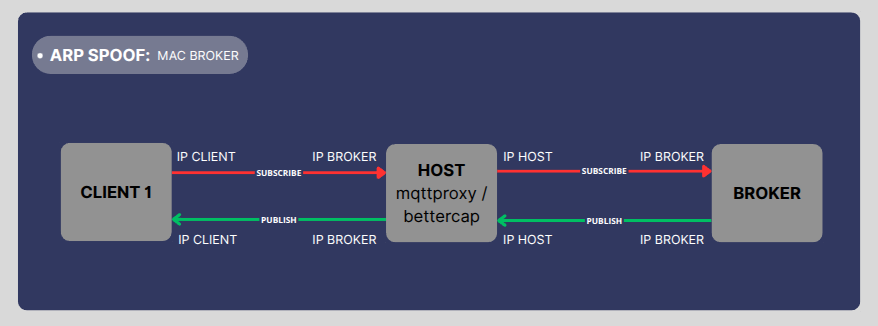
\includegraphics[width=1\textwidth]{img/mitmproxy.png}
    \caption{Esquema del trànsit generat per l'atac de Man In The Middle mitjançant un proxy TCP. S'observa que la connexió entre el client i el broker legítim no es trenca però si es canvien les respectives adreces IP.}
    \label{fig:MITMproxy}
  \end{figure}

  \begin{figure}[H]
    \centering
    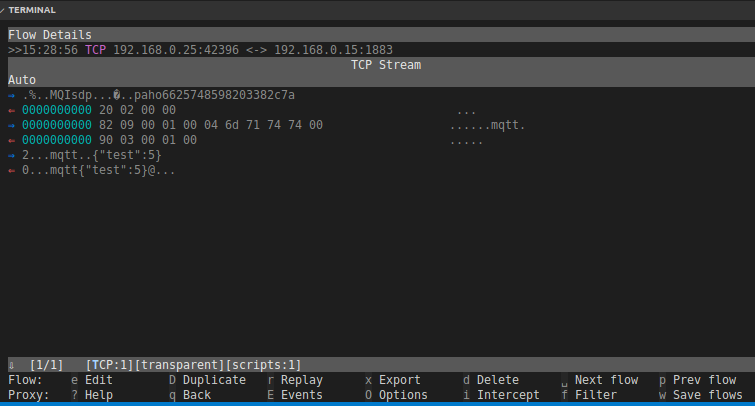
\includegraphics[width=1\textwidth]{img/mitmcapt.png}
    \caption{Captura de la interfície de mitmproxy on s'observa un trànsit TCP des de la IP 192.168.0.25 (client) a la IP 192.168.0.15 (broker).}
    \label{fig:MITMcapt}
  \end{figure}

Finalment, s'ha actualitzat la implementació anterior per tal que el proxy actuï com a proxy transparent. Això vol dir que el client i el broker no són conscients de la seva existència, ja que no es canvien les adreces IP dels missatges, sinó que el proxy simplement reenvia els missatges entre ambdues parts. Això permet que el trànsit MQTT flueixi sense interrupcions i fa que sigui més difícil detectar l'atac.

Per a què el proxy actuï com a proxy transparent, s'han utilitzat les següents regles de firewall IPTABLES:

\begin{lstlisting}[language=bash, caption={Execució iptables}, label=lst:iptables]
  iptables -t nat -A PREROUTING -p tcp --dport 1883 -j REDIRECT
  iptables -t nat -A POSTROUTING -p tcp --dport 1883 -j SNAT --to-source 192.168.0.41
  \end{lstlisting}

  Amb la primera regla s'especifica que tot el trànsit TCP que arriba al port 1883 (port per defecte MQTT) serà redirigit al proxy mitmproxy. La segona regla especifica que l'adreça IP d'origen dels missatges serà la del client legítim, fent que el broker legítim no pugui distingir entre el trànsit legítim i el trànsit interceptat pel proxy.

  Per a la implementació d'aquest atac, per tant, hem d'enverinar el trànsit ARP de forma bidireccional, és a dir, tant l'adreça MAC del client com la del broker han de ser substituïdes per l'adreça MAC de l'atacant.

  \begin{figure}[H]
    \centering
    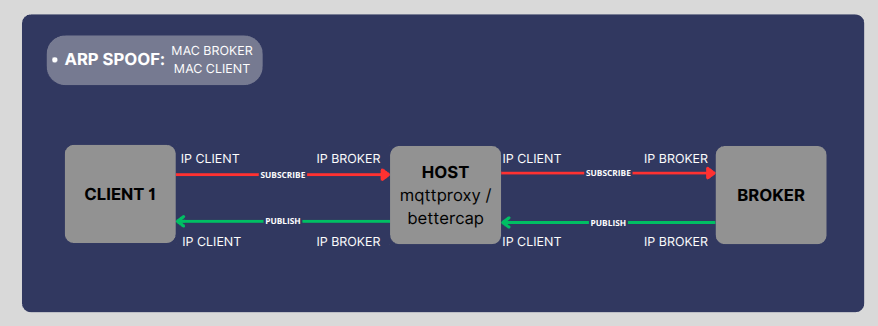
\includegraphics[width=1\textwidth]{img/mitmproxytransp.png}
    \caption{Esquema del trànsit generat per l'atac de Man In The Middle mitjançant un proxy TCP transparent. S'observa que la connexió entre el client i el broker legítim no es trenca ni es canvien les respectives adreces IP, donant un efecte de continuïtat en el flux de dades.}
    \label{fig:MITMproxyTransparent}
  \end{figure}

  Un cop implementats els atacs de MITM, s'ha utilitzat el motor d'scripting de mitmproxy per tal de manipular els missatges transmesos. Aquest motor permet escriure scripts en Python que poden modificar, enregistrar o bloquejar els missatges MQTT que passen pel proxy. Això obre la porta a una àmplia gamma de possibles atacs i manipulacions del trànsit MQTT, com ara la injecció de missatges maliciosos o la modificació de les dades transmeses. En aquest treball, s'ha implementat un script senzill que registra els missatges en direcció al client i en trobar un camp concret en format JSON, modifica el seu valor (codi: \ref{lst:ScriptMITM}). També s'ha implementat un segon script que mitjançant una modificació de baix nivell, modifica el cos del missatge MQTT Publish bit a bit, sigui quin sigui el seu contingut (codi: \ref{lst:ScriptMITM2}). Aquests scripts es poden afegir a l'execució del proxy mitmproxy amb el paràmetre \textit{-s}.

  De forma alternativa, també s'ha utilitzat Bettercap per a implementar l'atac d'ARP spoofing i MITM de forma unificada, però el seu motor d'scripting en JavaScript és molt més limitat i no perment manipular els missatges MQTT, ja que no té suport per aquest protocol de forma nativa ni permet la modificació a baix nivell.

  S'han testejat els scripts explicats anteriorment enviant missatges des de clients, en la següent figura es pot observar un missatge enviat a un servidor d'eco i la seva modificació a al missatge retornat. 
    \begin{figure}[H]
    \centering
    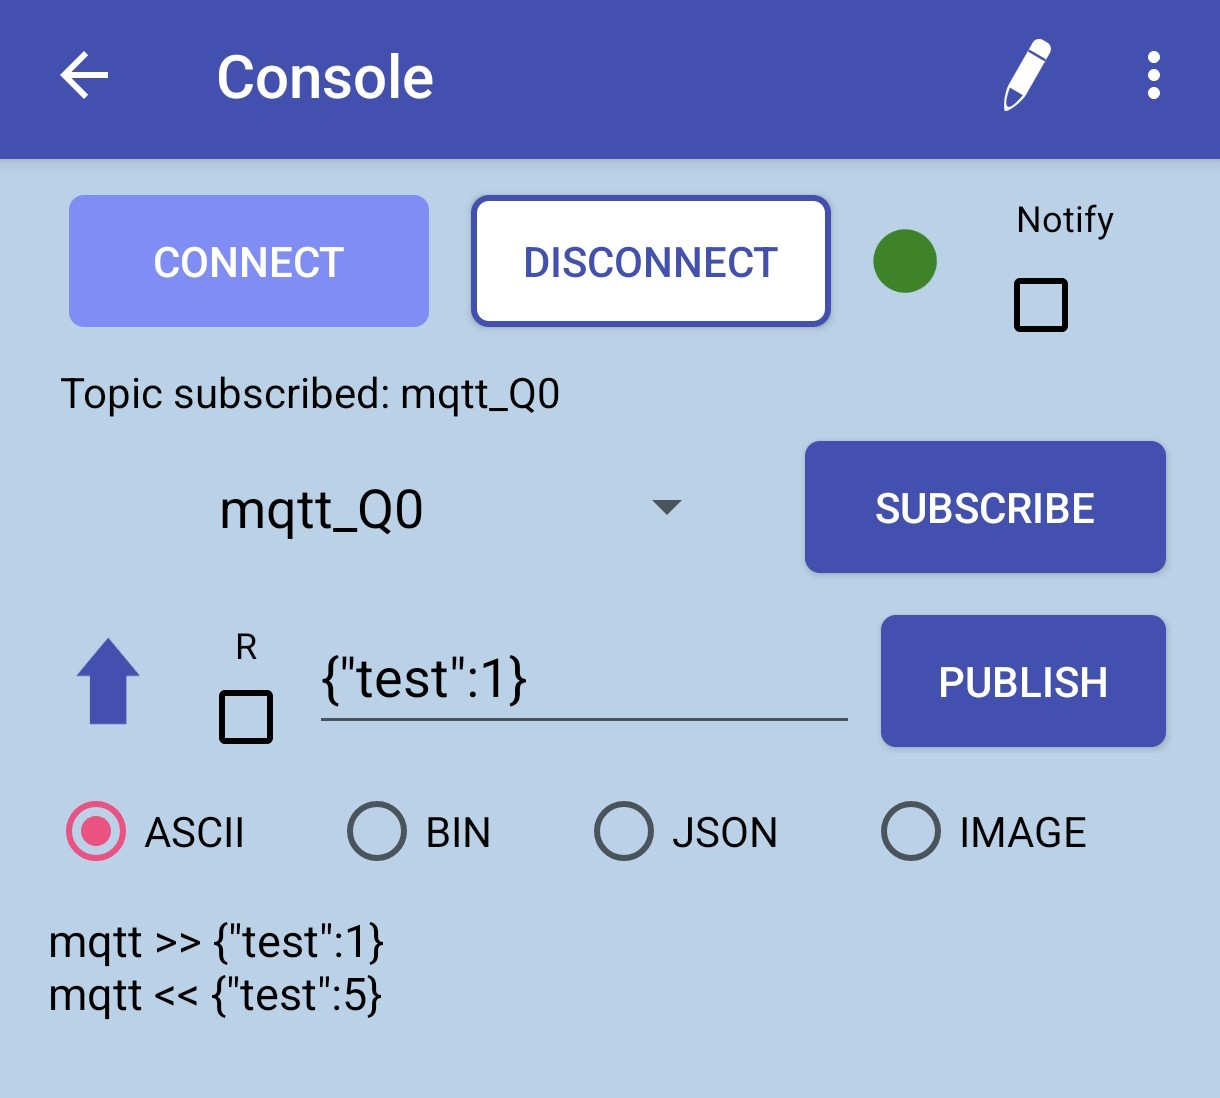
\includegraphics[width=0.7\textwidth]{img/captmqttclient.jpg}
    \caption{Captura de l'aplicació Android MQTT Terminal utilitzada com a client MQTT, es connecta al broker 192.168.0.15 (que està actuant com a servidor echo) passant pel proxy mitmproxy. S'observa un exemple de funcionament de l'script de modificació de trànsit al modificar el valor de la variable "test" enviada.}
    \label{fig:MqttClientCapt}
  \end{figure}